\section*{Question 1}

Consider an RBC model with a representative household that maximizes utility
$$U_t=E_t\sum_{t=0}^\infty\beta^t\left(\log\left(C_t\right)+\nu\left(1-L_t\right)\right)$$


where $\nu$ is an increasing and concave function. The production function is
$$Y_t=A_tL_t^{1-\alpha}\left(z_tK_t\right)^\alpha $$

with $0<\alpha<1$ and $z_t$ denotes a capital utilization choice. For example, low capital utilization may mean
running the machines only at half speed or half of the time.
Capital accumulation is described by

$$K_{t+1}=\left(1-\bar{\delta}z_t^\phi\right)K_t+Y_t-C_t.$$

\begin{problem*}[1]
    Explain how variable utilitzation of capital is modeled here. Should we assume that $\phi<1$ or $\phi>1?$
\end{problem*}

\begin{solution}
    \textcolor{blue}{
        In the given model, capital utilization $z_t$ directly affects both production and capital depreciation: in the production function, $z_t K_t$ is the effective capital input at time period $t$, higher $z_t$ increases the effective capital services, thus boosting output. The depreciation rate is $\delta_t = \bar{\delta}z_t^{\phi}$, and higher $z_t$ leads to a higher depreciation rate. \\
        Depreciation Function $\delta_t = \bar{\delta}z_t^{\phi}$ determines how sensitively depreciation responds to changes in utilization $z_t$.The marginal increase in depreciation due to higher $z_t$ is given by: 
        \[
        \frac{\partial \delta_t}{\partial z_t} = \bar{\delta}\phi z_t^{\phi-1}.
        \]
        Intuitively, if utilization increases, the marginal cost of utilizing capital rises, reflecting higher incremental damage, meaning that teh capital depreciates faster, which implies:
        \[
        \frac{\partial^2 \delta_t}{\partial z_t^2} = \bar{\delta}\phi(\phi-1) z_t^{\phi-2} > 0.
        \]
        Hence, we should assume that $\phi > 1.$
    }
\end{solution}

\begin{problem*}[2]
    Derive and explain the optimality conditions of the social planner's problem. 
    The social planner's problem is to maximize total utility subject to the economy's physical resource constraints 
    (i.e. production, and the law of motion for capital). 
    The social planner can set the levels of consumption, investment, capacity utilization, and labor supply, 
    without having to worry about prices or market clearing. 
\end{problem*}

\begin{solution}
    \textcolor{blue}{
        The social planner maximizes the expected discounted utility:
        \begin{align*}
            \max_{\{C_t, I_t, L_t, z_t\}} & E_t \sum_{t=0}^\infty \beta^t \left(\log(C_t) + \nu(1-L_t)\right) \\
            \text{s.t.} \quad & Y_t = A_t L_t^{1-\alpha} (z_t K_t)^\alpha \\
            \quad \quad & K_{t+1} = (1-\bar{\delta} z_t^\phi) K_t + Y_t - C_t
        \end{align*}
        Define the Lagrangian:
        \[ 
        \mathcal{L} = E_t \sum_{t=0}^\infty \beta^t \left\{\log(C_t) + \nu(1-L_t) - \lambda_t \left[C_t + K_{t+1} - (1-\bar{\delta} z_t^\phi) K_t - Y_t\right]\right\}
        \]
        The first-order conditions are:
        \begin{align}  
            & \frac{\partial \mathcal{L}}{\partial C_t} = \beta^t (\frac{1}{C_t}-\lambda_t) = 0 \Rightarrow \frac{1}{C_t} = \lambda_t \\
            & \frac{\partial \mathcal{L}}{\partial L_t} = \beta^t\left[-\nu'(1-L_t) + \lambda_t A_t (1-\alpha) L_t^{-\alpha} (z_t K_t)^\alpha \right] = 0 \Rightarrow \nu'(1-L_t) = \lambda_t A_t (1-\alpha) L_t^{-\alpha} (z_t K_t)^\alpha \\
            & \frac{\partial \mathcal{L}}{\partial z_t} = \beta^t \lambda_t \left[ A_t \alpha L_t^{1-\alpha} z_t^{\alpha-1} K_t^\alpha - \bar{\delta} \phi z_t^{\phi-1} K_t\right] = 0 \Rightarrow \bar{\delta} \phi z_t^{\phi-1} = A_t \alpha L_t^{1-\alpha} z_t^{\alpha-1} K_t^{\alpha-1}\label{(*)} \\
            & \frac{\partial \mathcal{L}}{\partial K_{t+1}} = -\beta^t \lambda_t + \beta^{t+1}\lambda_{t+1}\left[(1-\bar{\delta}z_{t+1}^{\phi}) + \alpha \frac{Y_{t+1}}{K_{t+1}}\right] = 0 \Rightarrow \lambda_t = \beta \lambda_{t+1} (1-\bar{\delta} z_{t+1}^\phi + \alpha \frac{Y_{t+1}}{K_{t+1}})\label{(**)}
        \end{align}
        From the FOCs, we could tell that:
        \begin{enumerate}
            \item The shadow price of consumption equals to the marginal utility of consumption.
            \item For the derivative with respect to $L_t$, we can transform it into the following format: \[
            \nu'(1-L_t) = \frac{\partial Y_t}{C_t \partial L_t}
            \]
            The marginal utility of leisure equals the marginal utility gain from increased consumption made possible by supplying an extra unit of labor.
            \item For the derivative with respect to $z_t$, we can transform it into the following format:
            \[
            \frac{\partial \delta_t K_t}{\partial z_t} = \frac{\partial Y_t}{\partial z_t}
            \]
            The marginal cost(depreciation) of capital equals to the marginal gain of production of increasing capital utilization.
            \item The standard inter-temporal condition balancing current and future utility.
        \end{enumerate}
    }
\end{solution}

\begin{problem*}[3]
    Derive an expression for the steady-state capital utilization $z^*$ in terms of the steady-state capital-output ratio. If we want to normalize $z^*=1$, how should we calibrate $\phi$?
\end{problem*}

\begin{solution}
    \textcolor{blue}{
        At the steady state: $Y_t = Y$, $C_t = C$, $K_t = K$, $A_t = A$ and $L_t = L$.
        Since $C_t = C_{t+1}$, we know that $\lambda_t = \lambda_{t+1}.$
        From \ref{(*)}, we know that:
        \begin{align*}
            \alpha A L^{1-\alpha} (z^* K)^{\alpha-1} & = \phi \bar{\delta }z^{*^{\phi -1}} = \frac{\alpha Y}{z^* K} \\
            \Rightarrow \frac{Y}{K} & = \frac{\phi \bar{\delta} z^{*^{\phi }}}{\alpha}
        \end{align*}
        Denote $\kappa = \frac{K}{Y}$, which is the output ratio, we would have:
        \[
        z^* = \left( \frac{\alpha}{\kappa \phi \bar{\delta} }\right)^{\frac{1}{\phi}}.  
        \]
        Then, we use \ref{(**)} and $\lambda_t = \lambda_{t+1}$, we'll have:
        \begin{align*}
            & 1 = \beta(1 - \bar{\delta}z^{*^{\phi}} + \alpha \frac{Y}{K}) = \beta(1- \bar{\delta}z^{*^{\phi}} +\alpha \frac{\phi \bar{\delta} z^{*^{\phi }}}{\alpha} ) = \beta(1- \bar{\delta}z^{*^{\phi}} + \phi \bar{\delta} z^{*^{\phi }}) \\
            \Rightarrow & (\phi-1)\bar{\delta} z^{*^{\phi}} = \frac{1-\beta}{\beta} \\
            \Rightarrow & z^* = \left(\frac{1-\beta}{\beta (\phi-1) \bar{\delta}}\right)^{\frac{1}{\phi}}
        \end{align*}   
        Normalize $z^* = 1$, we simplify the equation into:
        \[
        1 - \beta = \beta (\phi-1) \bar{\delta},
        \]
        which gives that
        \[
        \phi = \frac{1-\beta}{\beta \bar{\delta}} + 1 = \frac{1 - \beta + \beta \bar{\delta}}{\beta \bar{\delta}}
        \]
        Or, we would simplify the expression of $z^*$ with capital-output ratio $\kappa$:
        \[
        \alpha = \kappa \phi \bar{\delta} \Rightarrow \phi = \frac{\alpha}{\kappa \bar{\delta}}
        \]
    }
\end{solution}

\begin{problem*}[4]
    Compared to a standard RBC model (as in the lecture), do you expect this model to generate a
stronger or weaker response of output to a TFP shock?
\end{problem*}

\begin{solution}
    \textcolor{blue}{
        Compared to a standard RBC model, this model generates stronger response of output to a TFP shock.\\
        \textbf{In the Standard RBC Model:}\\
        Capital utilization is fixed ($z_t=1$). Output response to TFP shocks relies solely on adjustments in labor and capital.\\
        \textbf{In This Model with Variable Utilization:}\\
        Firms can adjust $z_t$ in response to TFP shocks.
        A positive TFP shock allows firms to temporarily increase $z_t$ , boosting output beyond what is possible in the standard model, which gives higher fluctuations.
    }
\end{solution}

\begin{problem*}[5]
    Assuming the model is correct, how is the standard empirical Solow residual $\log Y_t-(1-\alpha)\log L_t-\alpha\log K_{t}$ 
    related to total factor productivity $\log A_{t}$? 
\end{problem*}

\begin{solution}
    \textcolor{blue}{
        If our model is correct, then we log-linearize the production function:
    \begin{align*}
        & \log Y_t = \log A_t + (1-\alpha)\log L_t + \alpha \log K_t + \alpha \log z_t \\
        \Rightarrow & \text{Solow Residual} = \log Y_t - (1-\alpha)\log L_t - \alpha \log K_t = \log A_t + \alpha \log z_t
    \end{align*}
    }
\end{solution}

\section*{Question 2}

We study a variation of the simplified RBC model from the lecture. Consider an economy populated by a mass of representative households and a mass of representative firms which take output and factor prices as given. The production function is Cobb-Douglas:

$$Y_t=e^{z_t}K_t^\alpha L_t^{1-\alpha}$$

where $e^z_t$ is total factor productivity, $K$ is capital, and $L$ is labor. Capital fully depreciates in every
periods so that
$$K_{t+1}=I_t$$

where $I_{t}$ is investment.

The representative household supplies labor $L_t$ and consumes $C_t.$ It maximizes

$$U=E_0\left[\sum_{t=0}^\infty\beta^t\left[\log C_t-e^{\chi_t}L_t\right]\right]$$

where $\chi_t$ is a preference shock. Capital is accumulated by the household and rented to the firm, as usual.
Any profits of the firms are rebated to the households. As usual, we have $0<\alpha<1,0<\beta<1.$

\begin{problem*}[1]
    Write down the budget constraint of the household and the profit function of firms.
\end{problem*}

\begin{solution}
    \textcolor{blue}{
        Assume the rental rate of capital is $r_t$ and the wage rate is $w_t$.
        The budget constraint of the household is:
        \[
        C_t + K_{t+1} = r_t K_t + w_t L_t + \Pi_t
        \]
        The profit function of firms is:
        \[
        \Pi_t = Y_t - r_t K_t - w_t L_t = e^{z_t} K_t^\alpha L_t^{1-\alpha} - r_t K_t - w_t L_t
        \]
    }
\end{solution}

\begin{problem*}[2]
    Derive first-order conditions of firms and households.
\end{problem*}

\begin{solution}
    \textcolor{blue}{
        From problem (1), we established:
        \[ 
        \Pi_t = Y_t - r_t K_t - w_t L_t \Rightarrow r_t K_t + w_t L_t + \Pi_t = Y_t.
        \]
        Thus, our households budget constraint is:
        \[
        C_t + K_{t+1} = Y_t.
        \]
        We define the Lagrangian of the household problem as:
        \[
        \mathcal{L} = E_0 \sum_{t=0}^\infty \beta^t \left[\log C_t - e^{\chi_t} L_t - \lambda_t (C_t + K_{t+1} - Y_t)\right].
        \]
        The first-order conditions of households are:
        \begin{align*}
            & \frac{\partial \mathcal{L}}{\partial C_t} = \beta^t (\frac{1}{C_t} - \lambda_t) = 0 \Rightarrow \frac{1}{C_t} = \lambda_t \\
            & \frac{\partial \mathcal{L}}{\partial L_t} = \beta^t (-e^{\chi_t} + \lambda_t \frac{\partial Y_t}{\partial L_t}) = 0 \Rightarrow e^{\chi_t} = \lambda_t \frac{\partial Y_t}{\partial L_t}\\
            & \frac{\partial \mathcal{L}}{\partial K_{t+1}} = -\beta^t \lambda 
            _t + \beta^{t+1}E_t \lambda_{t+1} \frac{\partial Y_{t+1}}{\partial K_{t+1} } = 0 \Rightarrow \lambda_t = \beta \lambda_{t+1} E_t \frac{\partial Y_{t+1} }{\partial K_{t+1} }
        \end{align*}
        Let's compute $\frac{\partial Y_t}{\partial L_t}$ and $\frac{\partial Y_t}{\partial K_{t+1} }$:
        \begin{align*}
            & \frac{\partial Y_t}{\partial L_t} = e^{z_t} K_t^\alpha (1-\alpha) L_t^{-\alpha} = (1-\alpha) \frac{Y_t}{L_t} \\
            & \frac{\partial Y_{t+1} }{\partial K_{t+1} } = \alpha e^{z_{t+1} } K_{t+1}^{\alpha-1} L_{t+1}^{1-\alpha} = \alpha \frac{Y_{t+1} }{K_{t+1} }
        \end{align*}
        So, our households FOCs are:
        \begin{align}
            & \lambda_t = \frac{1}{C_t}\label{1.1} \\
            & e^{\chi_t} = \lambda_t (1-\alpha ) \frac{Y_t}{L_t} = \frac{(1-\alpha )Y_t}{C_t L_t}\label{1.2} \\
            & \lambda_t = \alpha \beta \lambda_{t+1} E_t \frac{Y_{t+1} }{K_{t+1} } \Rightarrow \frac{1}{C_t} = \alpha \beta E_t \frac{Y_{t+1} }{C_{t+1} K_{t+1} }\label{1.3}
        \end{align}
        The Lagrangian of the firm problem is:
        \[
        \max_{K_t, L_t} \Pi_t = e^{z_t} K_t^\alpha L_t^{1-\alpha} - r_t K_t - w_t L_t
        \]
        The first-order conditions of firms are:
        \begin{align}
            & \frac{\partial \Pi_t}{\partial K_t} = \alpha e^{z_t} K_t^{\alpha-1} L_t^{1-\alpha} - r_t = 0 \Rightarrow r_t = \alpha e^{z_t} K_t^{\alpha-1} L_t^{1-\alpha} = \alpha \frac{Y_t}{K_t}\label{1.4} \\
            & \frac{\partial \Pi_t}{\partial L_t} = (1-\alpha) e^{z_t} K_t^\alpha L_t^{-\alpha} - w_t = 0 \Rightarrow w_t = (1-\alpha) e^{z_t} K_t^\alpha L_t^{-\alpha} = (1-\alpha )\frac{Y_t}{L_t}\label{1.5}
        \end{align}
    }
\end{solution}

\begin{problem*}[3]
    Show that when factor markets and final good markets are competitive, firm profits are zero.
\end{problem*}

\begin{solution}
    \textcolor{blue}{
        The competitive equilibrium requires that the rental rate of capital equals the marginal product of capital and the wage rate equals the marginal product of labor:
    \begin{align*}
        & r_t = \alpha \frac{Y_t}{K_t}  \\
        & w_t = (1-\alpha) \frac{Y_t}{L_t}
    \end{align*}
    In this case, the profit function of firms becomes:
    \[
    \Pi_t = Y_t - \alpha \frac{Y_t}{K_t} K_t - (1-\alpha) \frac{Y_t}{L_t} L_t = 0.
    \]
    }
\end{solution}

\begin{problem*}[4]
    Solve the model and show that the process for output in a competitive equilibrium is
    $$y_t=z_t+\alpha y_{t-1}-(1-\alpha)\chi_t$$ 
    (where lowercase letters denote the log of the uppercase letter).
\end{problem*}

\begin{solution}
    \textcolor{blue}{
        From the production function FOC \ref{1.3}, we have:
        $\frac{1}{C_t} = \alpha \beta E_t \frac{Y_{t+1} }{K_{t+1}C_{t+1}}.$
        Since $Y_{t+1} = C_{t+1} + I_{t+1} = C_{t+1} + K_{t+2}$, We have: 
        \begin{align*}
            \frac{1}{C_t} &= \alpha \beta E_t \frac{C_{t+1} + K_{t+2}}{K_{t+1}C_{t+1}} \\
            \Rightarrow \frac{K_{t+1} }{C_t} &= \alpha \beta E_t \left(1 + \frac{K_{t+2} }{C_{t+1} }\right)
        \end{align*} 
        \textcolor{red}{According to the Banach's Fixed-point Theorem}, $x = \alpha \beta (1+x)$, and we can solve \[\frac{K_{t+1}}{C_t} = \frac{\alpha \beta }{1-\alpha \beta}.\]\\
        As $K_{t+1} = Y_t - C_t$, we have $K_{t+1} = \alpha \beta Y_t $ and $C_t = (1-\alpha \beta )Y_t$.
        Then, by \ref{1.2} and \ref{1.5}, we know that:
        \begin{align*}
            e^{\chi _t} &= \frac{(1-\alpha )Y_t}{C_t L_t} \\
            \Rightarrow e^{\chi _t} &= \frac{(1-\alpha )Y_t}{(1-\alpha \beta )Y_t L_t} = \frac{1-\alpha }{1-\alpha \beta } \frac{1}{L_t} \\
            \Rightarrow L_t &= \frac{1-\alpha }{1-\alpha \beta }e^{-\chi _t}
        \end{align*} 
        \[Y_t = e^{z_t}K_t^\alpha L_t^{1-\alpha} = e^{z_t}(\alpha \beta Y_{t-1} )^\alpha \left(\frac{1-\alpha }{1-\alpha \beta }e^{-\chi _t}\right)^{1-\alpha}\]
        The the log of both sides, we have:
        \begin{align*}
            \log Y_t &= z_t + \alpha \log (\alpha \beta ) + \alpha \log Y_{t-1} + (1-\alpha )\log \left(\frac{1-\alpha }{1-\alpha \beta }\right) - (1-\alpha )\chi _t \\
            &= z_t + \alpha \log Y_{t-1} - (1-\alpha )\chi _t + \alpha \log (\alpha \beta ) + (1-\alpha )\log \left(\frac{1-\alpha }{1-\alpha \beta }\right)\\
            \Rightarrow y_t &= z_t + \alpha y_{t-1} - (1-\alpha )\chi _t + \alpha \log (\alpha \beta ) + (1-\alpha )\log \left(\frac{1-\alpha }{1-\alpha \beta }\right)
        \end{align*}
        We drop the constant and gives: $y_t = z_t + \alpha y_{t-1} - (1-\alpha )\chi _t.$
    }
\end{solution}

\begin{problem*}[5]
    Assume $y_{-1}=0$ and $z_t=0$ for all $t$, and $\chi_t=0$ for all $t$ except that $\chi_0=1\%.$ Draw the time path
for $\chi_{t},z_{t}$,and $y_{t}.$ Explain why $y_{t}$ is persistent.
\end{problem*}

\begin{solution}
    \ 

    \textcolor{blue}{
        At time period 0, $y_0 = z_0 + \alpha y_{-1} - (1-\alpha )\chi _0 = 1\%(\alpha-1)$, and after time period 0, we have $z_t = 0$ and $\chi_t = 0$, thus $y_t = \alpha y_{t-1} = 1\% \alpha^t(\alpha -1).$ Then, we can draw the three graphs as below:
    }
    
    % Graph 1
    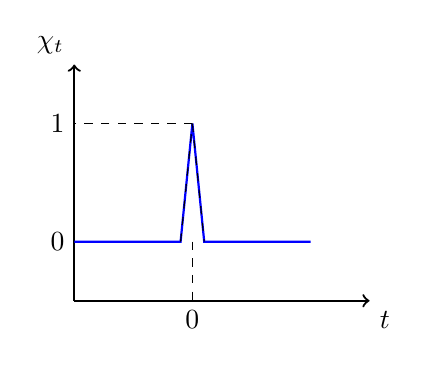
\begin{tikzpicture}[scale=1.5]
        % Axes
        \draw[thick,->] (0,0) -- (2.5,0) node[anchor=north west] {$t$};
        \draw[thick,->] (0,0) -- (0,2) node[anchor=south east] {$\chi _t$};
    
        % Plot
        \draw[thick, blue] (0,0.5) -- (0.9,0.5) -- (1,1.5) -- (1.1,0.5) -- (2,0.5);
    
        % Dashed lines
        \draw[dashed] (1,1.5) -- (0,1.5) node[anchor=east] {1};
        \draw[dashed] (1,0.5) -- (1,0) node[anchor=north] {0};
        \draw[dashed] (0.9,0.5) -- (1,1.5);
        \draw[dashed] (1,1.5) -- (1.1,0.5);
    
        % Labels
        % \node[below] at (1,0) {$0$};
        \node[left] at (0,0.5) {$0$};
    \end{tikzpicture}
        % Graph 2
    \begin{tikzpicture}[scale=1.5]
        \draw[thick,->] (0,0) -- (2.5,0) node[anchor=north west] {$t$};
        \draw[thick,->] (0,0) -- (0,2) node[anchor=south east] {$z_t$};
        \draw[thick, blue] (0,1) -- (2.2,1);
        \draw[dashed] (0,0.3) -- (0,0.3) node[anchor=east] {};
        \node[left] at (0,1) {0};
    \end{tikzpicture}
    % Graph 3
    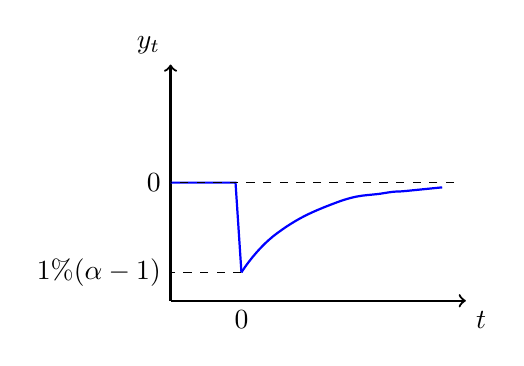
\begin{tikzpicture}[scale=1.5]
        \draw[thick,->] (0,0) -- (2.5,0) node[anchor=north west] {$t$};
        \draw[thick,->] (0,0) -- (0,2) node[anchor=south east] {$y_t$};
        \draw[thick, blue] (0,1) -- (0.55,1) -- (0.6,0.24);
        \draw[thick, blue] plot[smooth, tension=0.8] coordinates {(0.6,0.24) (0.9,0.57) (1.4,0.83) (1.8,0.91) (2.0, 0.93) (2.3,0.96)};
        \draw[dashed] (2.4,1) -- (0,1) node[anchor=east] {0};
        \draw[dashed] (0.6,0.24) -- (0,0.24) node[anchor=east] {$1\%(\alpha -1)$};
        \node[below] at (0.6,0) {0};
    \end{tikzpicture}
    
    \textcolor{blue}{
        The initial preference shock $\chi _0$ increases the disutility of labor, leading households to supply less labor at $t=0$. \\
        This reduces output at $t=0$.\\
        Since capital at $t+1$ depends on savings from $Y_t$ , the reduced output leads to lower capital $K_{t+1}$. \\
        The lower capital stock in subsequent periods reduces output further, even though the preference shock is gone.\\
        The capital accumulation process transmits the shock over time, causing persistence in output deviations from steady state.\\
        But as the shock has ended, the output will finally return back to the steady state.
    }
\end{solution}